All those sequencing techniques are aimed to investigate only one cellular compartment at a time, but in order to obtain a more comprehensive view of the cellular behaviour, it is necessary to look at more than one -omic at the same time.

\begin{figure}[h]
\centering
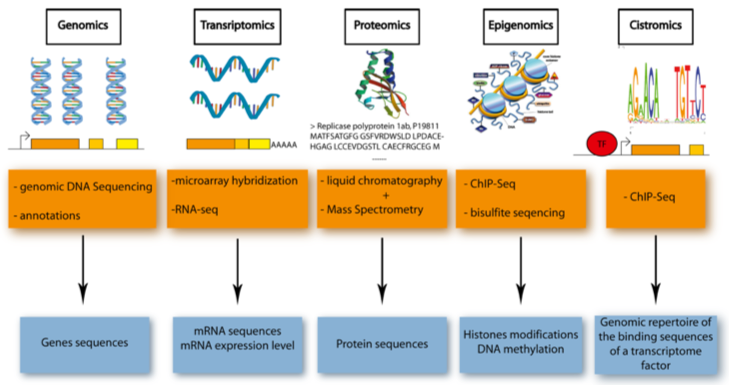
\includegraphics[width=8cm, keepaspectratio]{img/intro/omics.png}
\caption[Omics Representation]{}
\label{fig:omics}
\end{figure}

Indeed, we can imagine each omic as a camera in a multi-view camera system pointed on a building from different point of view.
Each device takes snapshots of the building from different angles, but the information is still fragmented.
In order to reconstruct a 3D model of the building, we need to put the snapshots took from each device together.

\begin{figure}[h]
\centering
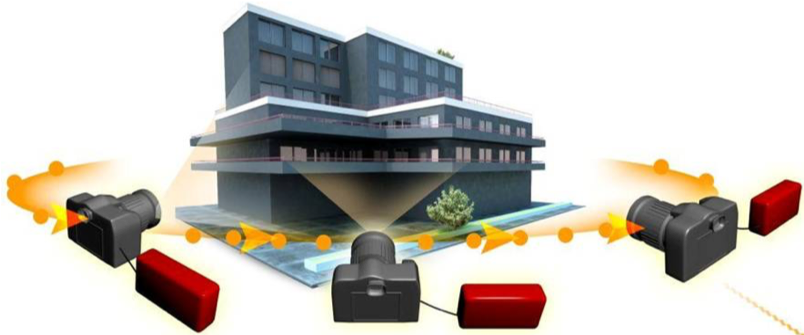
\includegraphics[width=8cm, keepaspectratio]{img/intro/cameras.png}
\caption[Integration cameras]{}
\label{fig:cameras}
\end{figure}

The same idea can be adapted to the sequencing techniques, we need to integrate information coming from different omics in order reconstruct (and understand) how multiple mechanisms orchestrate the cellular behavior.
As figure \ref{fig:funnell} outline, multi-omics data integration can be made at different levels, by graphical exploration, by functional annotation, by network fusion and by dimensionality reduction.

\begin{figure}[h]
\centering
\includegraphics[width=8cm, keepaspectratio]{img/intro/funnell.pdf}
\caption[Integration Funnell]{}
\label{fig:funnell}
\end{figure}

With graphical exploration, we can visualize data coming from different sources (e.g. \textit{RNA-seq} and \textit{ChIP-seq}) using specific tools designed at this scope, such as \textit{Genome Browser} \cite{Karolchik2011} or \gls{igv} \cite{Robinson2011, Thorvaldsdottir2013} and looking to the overlapping regions, or where expressed epigenomic markers have corrispondence with gene expression sites.


\textbf{CREATE SPECIFIC FIGURE FOR IGV OR GENOME BROWSER}




